\section{Polynomials}

Given a field \(\mathbb{K}\) and a variable \(x\), a \textit{polynomial} \(P\) of \(\mathbb{K}[x]\) is defined as a linear combination of powers of \(x\).
%
\[P = a_n x^n + a_{n-1} x^{n-1} + \cdots + a_2 x^2 + a_1 x + a_0 \tag{assuming \(a_n \neq 0\)}\]
%
Note that
%
\begin{itemize}
    \item The numbers \(a_i\) should all belong to the field \(\mathbb{K}\). They are called \textit{coefficients}.
    \item The products \(a_i x^i\) are called \textit{terms}.
    \item Here, \(n\) is the highest power in \(P\). This is known as the \textit{degree} of the polynomial.
\end{itemize}

Examples of polynomials include
%
\[x^2 \tag{degree \(2\)}\]
\[y - 1.5y^3 + 2 \tag{degree \(3\)}\]
\[z + 3z^4 \tag{degree \(4\)}\]
%
Although any symbol can be used to denote the variable of a polynomial, we will most use the letter \(x\) in this section.

A polynomial of degree \(0\) is simply a constant. On the other hand, a polynomial of degree \(1\), such as \(2x + 1\), is said to be \textit{linear}.


\subsection{Polynomials are not functions}

One important distinction to make is that technically speaking, polynomials are not functions:
%
\begin{itemize}
    \item A \textit{polynomial} is a strictly algebraic object. It is sometimes represented as a vector in a vector space. (We will further explore this idea below.)
    \item A \textit{function} is a mapping --- a rule that maps elements from a set to elements of another set.
    \item A \textit{polynomial function} is a specific type of function. While there is a one-to-one correspondence between polynomials and polynomial functions, they do not refer to the same idea.
\end{itemize}

Despite this, polynomials can be evaluated by substituting the variable with a value. For example, given the polynomial \(P = x^2 - 5x\), we can substitute \(x = 7\) to get
%
\[P(7) = 7^2 - 5 \times 7 = 14\text{.}\]



\subsection{Addition, multiplication and division of polynomials}

Polynomials can be added by summing up their like terms.
%
\begin{align*}
    (7x^3 + 8x^2 + 3) + (2x^2 + 9x - 4) &= 7x^3 + (8x^2 + 2x^2) + 9x + (3 - 4)\\
    &= 7x^3 + 10x^2 + 9x - 1
\end{align*}

Polynomials can also be multiplied by an element of \(\mathbb{K}\).
%
\[2(7x^3 + 8x^2 + 3) = 14x^3 + 16x^2 + 6\]

Let \(\mathbb{K}_n [x]\) be the set of all polynomials with coefficients in \(K\) and of degree at most \(n\). Since this set is closed under addition and scaling, it is a vector space.

We can multiply two polynomials by using expansion via distributivity.
%
\begin{align*}
    (8x + 3)(9x - 4) &= (8x)(9x) + (8x)(-4) + (3)(9x) + (3)(-4)\\
    &= 72x^2 - 32x + 27x - 12\\
    &= 72x^2 - 5x - 12
\end{align*}

If we denote the degree of a polynomial \(P\) as \(\deg(P)\), then:
%
\begin{align*}
    \deg(P + Q) &\leq \max(\deg(P) + \deg(Q)) \tag{highest-degree terms may cancel out}\\
    \deg(P \times Q) &\leq \deg(P) + \deg(Q)
\end{align*}

The fact that we can multiply polynomials implies that polynomials can have \textit{factors} --- for instance, we say that the polynomial \(72x^2 - 5x - 12\) has factors \(8x + 3\) and \(9x - 4\).

A polynomial with no non-constant factors is said to be \textit{irreducable}\footnote{This is analogous to how prime numbers work.}. For example, \(7x + 4\) is irreducable, but the following polynomials are not.
%
\begin{align*}
    x^2 + 7x + 12 &= (x+4)(x+3)\\
    x^3 + x^2 + 2x + 2 &= (x^2+2)(x+1)
\end{align*}
%
A polynomial is said to \textit{split} if it has only linear factors. Therefore, of the two polynomials listed above, the first one splits but the second one doesn't.

Lastly, we can perform division on polynomials, as explained below.
%
\begin{quote}
    \textbf{Euclidean division of polynomials.}

    Given two polynomials \(A\) and \(B\), there exists polynomials \(Q\) and \(R\) such that
    %
    \[A = QB + R\]
    %
    where \(R\) has a lower degree than \(B\). Here,
    %
    \begin{itemize}
        \item \(A\) is the dividend and \(B\) is the divisor.
        \item \(Q\) is the quotient and \(R\) is the remainder.
    \end{itemize}
\end{quote}

Given a dividend and a divisor, we can use long division to identify the corresponding quotient and remainder. An example of this is given in \ref{fig:Ch08-PolynomialDivision}, with the division
%
\[x^3 - 2x^2 - 4 = (x^2 + x + 3)(x - 3) + 5\text{.}\]
%
Note how the remainder (\(R = 5\)) has a lower degree than the divisor \(B = x - 3\).

\begin{figure}[H]
    \centering
    \includegraphics[width=0.3\linewidth]{Images/PolynomialDivision.png}
    \caption{An example of performing long division on polynomials.}
    \label{fig:Ch08-PolynomialDivision}
\end{figure}



\subsection{Roots of polynomials}

A number \(a\) in \(\mathbb{K}\) is said to be a root of a polynomial \(P\) if \(P(a) = 0\).

For example,
%
\begin{itemize}
    \item The linear polynomial \(P = 5x + 2\) has the root \(x = -2/5\) because \(P(-2/5) = 5(-2/5) + 2 = 0\).
    \item The polynomial \(Q = x^2 + 3x + 2\) has a root \(x = -2\) because \(Q(-2) = (-2)^2 + 3(-2) + 2 = 0\).
\end{itemize}

We now introduce the \textit{factor theorem}, which is illustrated below.
%
\begin{quote}
    \textbf{Factor theorem.} A number \(a\) is a root of a polynomial \(P\) if and only if \((x - a)\) is a factor of \(P\).

    \textbf{Proof.} We prove this statement in two directions.

    \((\Leftarrow)\): 
    %
    \begin{align*}
        (x-a) \text{ is a factor of } P &\implies P = (x-a)Q \hspace{3em} \text{for some polynomial } Q\\
        &\implies P(a) = (a - a)Q\\
        &\implies P(a) = 0\\
        &\implies a \text{ is a root of } P
    \end{align*}

    \((\Rightarrow)\): Assume \(a\) is a root of \(P\), so \(P(a) = 0\).
    
    We divide \(P\) by \(x - a\). By Euclidean division, there exists a polynomial \(Q\) and a constant \(r\) such that
    %
    \[P = Q \cdot (x-a) + r\text{.}\]
    
    (Recall that the remainder must have a lower degree than the  divisor \(x-a\). Since the divisor \((x - a)\) has degree \(1\), the remainder must be a constant with degree \(0\).)

    We evaluate both sides of the equation with \(x = a\).
    %
    \begin{align*}
        P(a) &= Q(a) \cdot (a-a) + r\\
        P(a) &= r\\
        r &= 0
    \end{align*}
    %
    Hence \(P = Q\cdot (x - a)\), so \(x - a\) is a factor of \(P\).
\end{quote}

This theorem is extremely useful for finding the roots of a polynomial. For instance, we can factor the polynomial
%
\begin{align*}
    2x^3 - x^2 - 8x + 4 &= x^2(2x-1) - 4(2x-1)\\
    &= (x^2 - 4)(2x - 1)\\
    &= (x+2)(x-2)(2x-1)\\
    &= 2(x+2)(x-2)\left(x-\frac{1}{2}\right)
\end{align*}
%
to show that it has the roots \(-2\), \(2\) and \(1/2\). But are these the only roots?

Yes, they are. We can prove this using the following theorem.
%
\begin{quote}
    \textbf{Theorem.} The number of roots\footnote{In this case, identical roots are counted separately. For example, the polynomial \(x^2 - 2x + 1 = (x-1)^2\) is treated as having two roots, both of value \(2\). We will dive deeper into this technicality later in this section when we talk about the multiplicity of a root.} of a polynomial in \(\mathbb{K}\) cannot exceed its degree.

    \textbf{Proof.} We label the roots of a polynomial \(P\) as \(r_1,\; r_2,\; r_3,\; \cdots,\; r_n\). Hence, by the factor theorem, we have
    %
    \begin{align*}
        P &= (x - r_1)(x - r_2)(x - r_3)\cdots(x - r_n) Q \tag{for some polynomial \(Q\)}\\
        \deg(P) &= \deg((x - r_1)(x - r_2)(x - r_3)\cdots(x - r_n) Q)\\
        &= n + \deg(Q)\\
        &> n
    \end{align*}
    %
    Therefore \(n < \deg(P)\).
\end{quote}

Note that the theorem above implies that the number of roots of a polynomial in \(\mathbb{K}\) may not necessarily equal its degree. To see why this is, we will have to take a closer look at polynomials of degree \(2\).



\subsection{On the real roots of polynomials of degree 2}

The simplest polynomial of degree \(2\) takes the form \(P = x^2 - a\). Finding its roots is equivalent to solving the equation
%
\[x^2 = a\]
%
which has the solutions \(\sqrt{a}\) and \(-\sqrt{a}\).

In general, however, a polynomial of degree \(2\) takes the form \(ax^2 + bx + c\). The corresponding function \(f(x) = ax^2 + bx + c\) is quadratic --- its graph is a parabola. The roots of the polynomial correspond to the points where the graph crosses the \(x\)-axis. See figures \ref{fig:Ch08-degree2-2roots}, \ref{fig:Ch08-degree2-1root} and \ref{fig:Ch08-degree2-0roots}.

\begin{figure}[H]
    \centering

    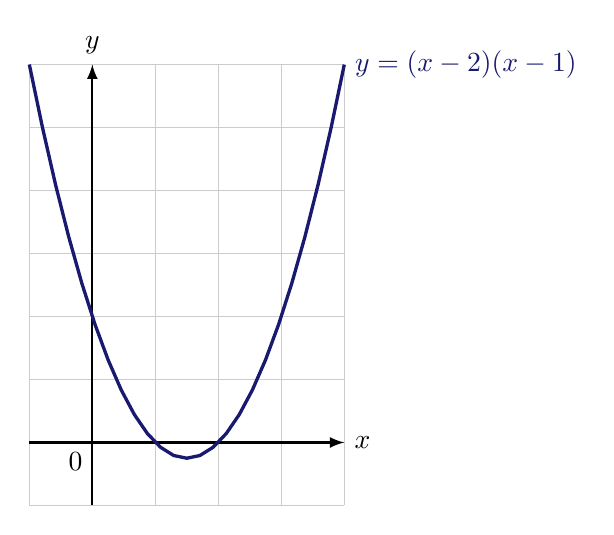
\begin{tikzpicture}[scale=0.8]
        \draw[thin,gray!40] (-1,-1) grid (4, 6);
        \draw[thick, ->, >=latex] (-1,0)--(4,0) node[right]{\(x\)};
        \draw[thick, ->, >=latex] (0,-1)--(0,6) node[above]{\(y\)};
        \draw (0, 0) node[below left] {0};

        \draw [MidnightBlue, very thick, domain=-1:4] plot (\x,{(\x)^2-(3*\x)+2}) node[right, MidnightBlue] {\(y = (x-2)(x-1)\)};

    \end{tikzpicture}
    
    \caption{An example of a polynomial of degree \(2\) with \(2\) distinct roots. The corresponding function has a graph has two \(x\)-intercepts.}
    \label{fig:Ch08-degree2-2roots}
\end{figure}

\begin{figure}[H]
    \centering

    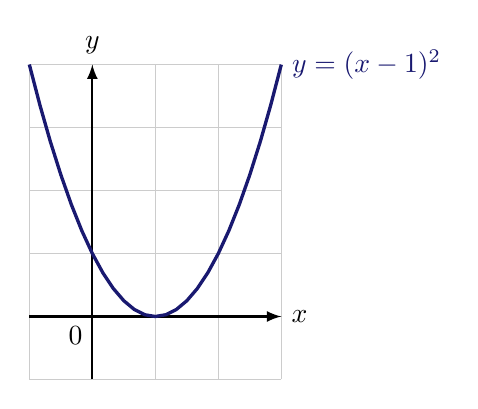
\begin{tikzpicture}[scale=0.8]
        \draw[thin,gray!40] (-1,-1) grid (3, 4);
        \draw[thick, ->, >=latex] (-1,0)--(3,0) node[right]{\(x\)};
        \draw[thick, ->, >=latex] (0,-1)--(0,4) node[above]{\(y\)};
        \draw (0, 0) node[below left] {0};

        \draw [MidnightBlue, very thick, domain=-1:3] plot (\x,{(\x-1)^2}) node[right, MidnightBlue] {\(y = (x-1)^2\)};

    \end{tikzpicture}
    
    \caption{An example of a polynomial of degree \(2\) with \(1\) root. The corresponding function has a graph has one \(x\)-intercept.}
    \label{fig:Ch08-degree2-1root}
\end{figure}

\begin{figure}[H]
    \centering

    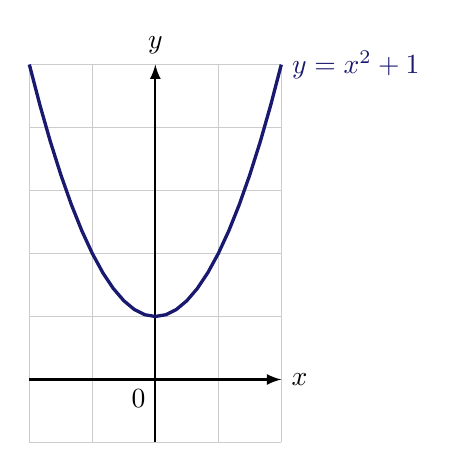
\begin{tikzpicture}[scale=0.8]
        \draw[thin,gray!40] (-2,-1) grid (2, 5);
        \draw[thick, ->, >=latex] (-2,0)--(2,0) node[right]{\(x\)};
        \draw[thick, ->, >=latex] (0,-1)--(0,5) node[above]{\(y\)};
        \draw (0, 0) node[below left] {0};

        \draw [MidnightBlue, very thick, domain=-2:2] plot (\x,{(\x)^2 + 1}) node[right, MidnightBlue] {\(y = x^2 + 1\)};

    \end{tikzpicture}
    
    \caption{An example of a polynomial of degree \(2\) with no roots in \(\mathbb{R}\). The corresponding function has a graph has no \(x\)-intercepts.}
    \label{fig:Ch08-degree2-0roots}
\end{figure}

Usually, we want to work out the number of roots of a polynomial of degree 2 without plotting its graph. This can be done by analysing its \textit{discriminant}. For a polynomial \(P = ax^2 + bx + c\), its determinant is defined as \(\Delta = b^2 - 4ac\).
%
\begin{itemize}
    \item If \(\Delta > 0\), then \(P\) has two distinct roots in \(\mathbb{R}\) and can be factored into the form \(P = a(x - r_1)(x - r_2)\).
    \item If \(\Delta = 0\), then \(P\) has one root\footnote{This is technically two non-distinct roots.} in \(\mathbb{R}\) and can be factored into the form \(P = a(x - r)^2\).
    \item If \(\Delta < 0\), then \(P\) has no roots in \(\mathbb{R}\) and is irreducable.
\end{itemize}
%
In the first two cases, the root(s) of \(P\) are given by the quadratic formula, as shown below.
%
\[x = \frac{-b \pm \sqrt{\Delta}}{2a} = \frac{-b \pm \sqrt{b^2 - 4ac}}{2a}\]



\subsection{On the complex roots of polynomials of degree 2}

If we allow complex roots, then a polynomial of degree \(2\) always have two (not necessarily distinct) roots \(r_1\) and \(r_2\) in \(\mathbb{C}\), as given by the quadratic formula. In other words, every polynomial of degree \(2\) splits in \(\mathbb{C}\) and can be factored into the form \(a(x-r_1)(x-r_2)\).

The two roots of a degree 2 polynomial
%
\begin{align*}
    r_1 &= \frac{-b + \sqrt{\Delta}}{2a} = \frac{-b + \sqrt{b^2 - 4ac}}{2a}\\
    r_2 &= \frac{-b + \sqrt{\Delta}}{2a} = \frac{-b - \sqrt{b^2 - 4ac}}{2a}
\end{align*}
%
are complex conjugates. This is proved below.
%
\begin{quote}
    \textbf{Theorem.} The two roots of a degree 2 polynomial must be complex conjugates.

    \textbf{Proof.} If \(\Delta \geq 0\), then both roots are real and therefore must be conjugates in \(\mathbb{C}\).

    If \(\Delta < 0\), then \(\sqrt{\Delta}\) is purely imaginary and can be expressed as \(di\) for some \(d \in \mathbb{R}\). Hence,
    %
    \begin{align*}
        r_1 &= \frac{-b + \sqrt{\Delta}}{2a} = \frac{-b + di}{2a} = \frac{-b}{2a} + \frac{d}{2a}i\\
        r_2 &= \frac{-b + \sqrt{\Delta}}{2a} = \frac{-b - di}{2a} = \frac{-b}{2a} - \frac{d}{2a}i
    \end{align*}
    %
    are complex conjugates.
\end{quote}
%
For example, the polynomial \(x^2 + 1\) has no real roots but can be factored in \(\mathbb{C}\) as \((x - i)(x + i)\). Its roots, \(i\) and \(-i\), are complex conjugates.

Below shows three useful identities for factoring polynomials of degree \(2\).
%
\begin{align*}
    (a+b)^2 &= a^2 + b^2 + 2ab\\
    (a-b)^2 &= a^2 + b^2 - 2ab\\
    (a+b)(a-b) &= a^2 - b^2
\end{align*}



\subsection{On the roots of polynomials of arbitrary degree}

We introduce the following theorems for polynomials of abritrary degree.

\begin{itemize}
    \item \textbf{Theorem on factorisations in \(\mathbb{R}\).}
    
    In \(\mathbb{R}\), only polynomials of degree \(2\) are irreducable\footnote{Note that it is still possible for polynomials of degree greater than \(2\) to have no real roots. This occurs when they are made entirely of irreducable quadratic factors. For example, the polynomial \(x^4 + 1\) can be factored into \(x^4 + 2x^2 + 1 - 2x^2 = (x^2 + 1)^2 - (\sqrt{2} x)^2 = (x^2 + 2\sqrt{x} + 1)(x^2 - 2\sqrt{x} + 1).\)}. Therefore, every polynomial \(P \in \mathbb{R}[x]\) of degree \(n > 0\) has a unique factorisation in \(\mathbb{R}\) of the form
    %
    \[P = {\color{BrickRed} c} {\color{OliveGreen} \underbrace{(x - \lambda_1)(x - \lambda_2) \cdots (x-\lambda_m)}_{\text{linear factors}}} {\color{MidnightBlue} \underbrace{(x^2 + a_1 x + b_1)(x^2 + a_2 x + b_2) \cdots (x^2 + a_k x + b_k)}_{\text{quadratic factors}}}\]
    %
    where
    %
    \begin{itemize}
        \item the constants \({\color{BrickRed} c},\; {\color{OliveGreen} \lambda_1,\; \lambda_2,\; \cdots,\; \lambda_m},\; {\color{MidnightBlue} a_1,\; a_2,\; \cdots a_k,\; b_1,\; b_2,\; \cdots b_k}\) are real numbers.
        \item Each quadratic factor is irreducable with a negative determinant, i.e. \(\Delta_i = a_i^2 - 4b_i < 0\) for \(1 \leq i \leq k\).
    \end{itemize}

    \item \textbf{Theorem on factorisations in \(\mathbb{C}\).}
    
    Each polynomial \(P \in \mathbb{R}[x]\) of degree \(n > 0\) has a unique factorisation in \(\mathbb{C}\) of the form
    %
    \[P = c(x - \lambda_1)(x - \lambda_2) \cdots (x-\lambda_n)\]
    %
    where \(c, \lambda_1,\; \lambda_2,\; \cdots,\; \lambda_n \in \mathbb{C}\).
    
    In other words, every real polynomial splits in \(\mathbb{C}\) with \(n\) (not necessarily distinct) complex roots \(\lambda_1,\; \lambda_2,\; \cdots,\; \lambda_n\).
\end{itemize}

When roots are not distinct, a polynomial can be written as
%
\[P = c (x - \lambda_1)^{k_1} (x - \lambda_2)^{k_2} (x - \lambda_3)^{k_3} \cdots (x - \lambda_j)^{k_j}\]
%
where \(k_1,\; k_2,\; k_3,\; \cdots,\; k_j \geq 1\). We say that \(k_i\) is the \textit{multiplicity} of \(\lambda_i\).



\subsection{A theorem on real polynomials of odd degrees}

Finally, we introduce an interesting theorem regarding real polynomials of odd degrees.

\begin{quote}
    \textbf{Theorem.} Any polynomial \(P\) of odd degree and with real coefficients has at least one real root.

    \textbf{Proof 1: An algebraic proof.} We first prove the following lemma: If \(z\) is a complex and non-real root of \(P\), then so is its conjugate \(\bar{z}\).
    
    We write \(P\) as follows:
    %
    \[P = {\color{BrickRed} c} {\color{OliveGreen} \underbrace{(x - \lambda_1)(x - \lambda_2) \cdots (x-\lambda_m)}_{\text{linear factors}}} {\color{MidnightBlue} \underbrace{(x^2 + a_1 x + b_1)(x^2 + a_2 x + b_2) \cdots (x^2 + a_k x + b_k)}_{\text{quadratic factors}}}\]
    %
    where the constants \({\color{BrickRed} c},\; {\color{OliveGreen} \lambda_1,\; \lambda_2,\; \cdots,\; \lambda_m},\; {\color{MidnightBlue} a_1,\; a_2,\; \cdots a_k,\; b_1,\; b_2,\; \cdots b_k}\) are real numbers; and each quadratic factor is irreducable with a negative determinant.

    We assume \(z\) is a root of \(P\), which means that \((x - z)\) is a factor. Since \(z \notin \mathbb{R}\), we have \(z \neq \lambda_1,\; \lambda_2,\; \cdots,\; \lambda_m\). Hence, \((x - z)\) must be a factor of one of the quadratic factors, i.e. \((x^2 + a_j x + b_j)\) where \(1 \leq j \leq k\).

    We know that the two roots of a quadratic polynomial are always complex conjugates. Therefore, \((x - \bar{z})\) is also a factor of \((x^2 + a_j x + b_j)\).

    This means that \((x - \bar{z})\) is a factor of \(P\), so \(\bar{z}\) is a root of \(P\). This concludes the proof for the lemma.

    We now prove the required theorem. Since \(P\) has an odd degree, it must also have an odd number of roots. By the previously proved lemma, for any complex and non-real root \(z\) of \(P\), its conjugate \(\bar{z} \neq z\) is also a root. Hence, the number of non-real roots of \(P\) must be even. This means that the number of real roots of \(P\) must be odd, i.e. at least one. Hence proved.

    \textbf{Proof 2: A calculus proof.} We write \(P\) as follows:
    %
    \[P = a_n x^n + a_{n-1} x^{n-1} + \cdots + a_1 x + a_0\]
    %
    where \(n\) is odd and \(a_n \neq 0\). We will dissect the proof into two cases.

    In the first case, we have \(a_n > 0\). Notice that as \(x\) approaches positive infinity, so does \(P\). This means that
    %
    \[\forall d > 0, \exists c > 0, x > c \implies P(x) > d\text{.}\]
    %
    Substituting \(d = 1\) (or any positive value) tells us that there exists some positive constant \(c\) such that \(x > c \implies P(x) > 1\). This means that there exists some \(x_{\text{pos}}\) for which \(P(x_{\text{pos}})\) is positive.

    Similarly, notice that as \(x\) approaches negative infinity, so does \(P\) (since \(n\) is odd). This means that
    %
    \[\forall d < 0, \exists c < 0, x > c \implies P(x) < d\text{.}\]
    %
    Substituting \(d = -1\) (or any negative value) tells us that there exists some negative constant \(c\) such that \(x < c \implies P(x) < -1\). This means that there exists some \(x_{\text{neg}}\) for which \(P(x_{\text{neg}})\) is negative.

    Combining the two results above with the intermediate value theorem, we see that there must exist some value \(x_0\) such that \(x_{\text{neg}} < x_0 < x_{\text{pos}}\) and \(P(x_0) = 0\). This \(x_0\) is a real root of \(P\). Hence proved.
\end{quote}
